%----------------------------------------------------------------------------------------
%	PACKAGES AND OTHER DOCUMENT CONFIGURATIONS
%----------------------------------------------------------------------------------------

\documentclass[
	11pt, 
	%aspectratio=169, 
]{beamer}

\graphicspath{{../assets/proposal/}{./}} % Specifies where to look for included images

\usepackage{booktabs} 
\usepackage[utf8]{inputenc}
% \usepackage[T5]{fontenc} % Bỏ comment dòng này nếu dùng pdflatex để biên dịch tiếng Việt. Khuyên dùng XeLaTeX.

%----------------------------------------------------------------------------------------
%	SELECT LAYOUT THEME
%----------------------------------------------------------------------------------------

\usetheme{Madrid}

%----------------------------------------------------------------------------------------
%	SELECT FONT THEME & FONTS
%----------------------------------------------------------------------------------------

\usefonttheme{default}
\usepackage[default]{opensans}

%----------------------------------------------------------------------------------------
%	SELECT INNER THEME
%----------------------------------------------------------------------------------------

\useinnertheme{circles}

% Tắt thanh điều hướng (các nút nhỏ ở góc dưới)
\setbeamertemplate{navigation symbols}{}

%----------------------------------------------------------------------------------------
%	PRESENTATION INFORMATION
%----------------------------------------------------------------------------------------

\title[Đồ án cuối kỳ]{ĐÁNH GIÁ VÀ HIỆU CHÍNH TÍNH NHẤT QUÁN HÌNH HỌC 3D CHO ƯỚC LƯỢNG ĐỘ SÂU VIDEO BẰNG VGGT}

\subtitle{VGGT-GUIDED EVALUATION AND TEST-TIME ADAPTATION}

\author[Nguyễn Lưu Trọng Tấn]{Nguyễn Lưu Trọng Tấn - 250201089} 

\institute[UIT]{Trường Đại học Công nghệ Thông tin - ĐHQG TP.HCM (UIT)}

\date[\today]{\today}

%----------------------------------------------------------------------------------------

\begin{document}

% SLIDE 1
\begin{frame}
	\titlepage 
\end{frame}

% SLIDE 2
\begin{frame}
	\frametitle{Tóm tắt thông tin}
	
	\begin{itemize}
		\item \textbf{Lớp:} CS2205.JAN2026
		\item \textbf{Link Github:} \textit{[để trống]}
		\item \textbf{Link Youtube:} \textit{[để trống]}
		\item \textbf{Ảnh + Họ và tên:} \textit{[để trống]}
	\end{itemize}
\end{frame}

%----------------------------------------------------------------------------------------

\section{Giới thiệu}

% SLIDE 3
\begin{frame}
	\frametitle{Giới thiệu - Đặt vấn đề}
	
	\begin{itemize}
		\item \textbf{Bối cảnh:} Ước lượng độ sâu từ video đóng vai trò quan trọng trong robot, xe tự hành, thực tế tăng cường và định vị camera.
		\item \textbf{Vấn đề:}
		\begin{itemize}
			\item Các mô hình hiện đại (như Depth Anything V2, Video Depth Anything) đã cải thiện độ ổn định hình ảnh, nhưng \alert{chưa đồng nghĩa với nhất quán hình học 3D}.
			\item Bản đồ độ sâu có thể thay đổi trơn tru theo thời gian nhưng vẫn bị trôi tỉ lệ, sai lệch khi camera di chuyển hoặc làm biến dạng vật thể 3D.
			\item Các chỉ số cũ (AbsRel, RMSE) chủ yếu đánh giá trên từng khung hình, không phản ánh được các sai lệch tích lũy này.
		\end{itemize}
	\end{itemize}
	
	\begin{figure}
		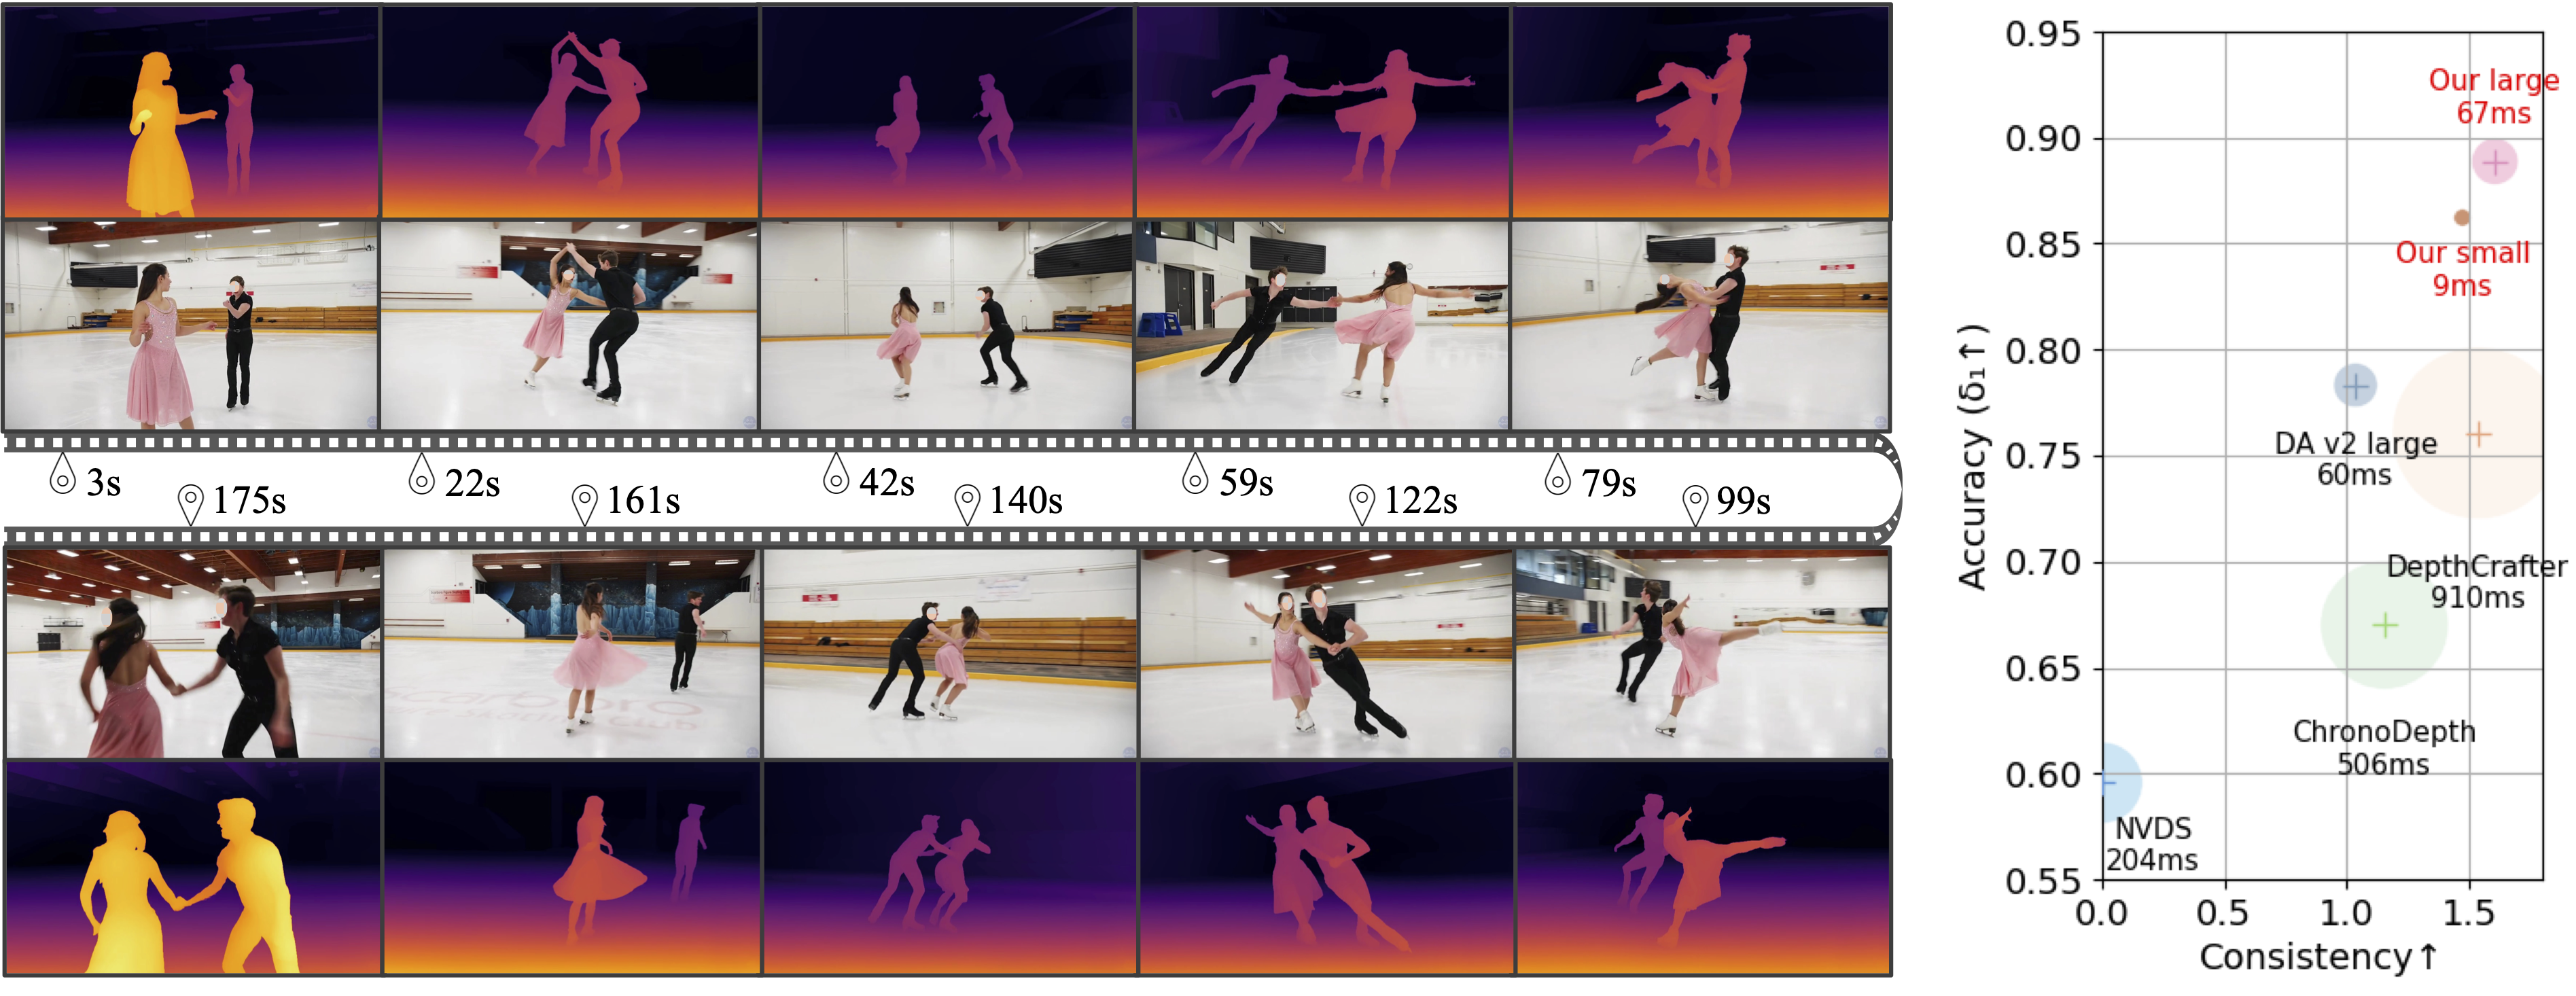
\includegraphics[width=0.55\linewidth]{video_depth_anything_teaser.png}
		\caption{Minh họa Video Depth Anything hướng tới độ sâu ổn định thời gian.}
	\end{figure}
\end{frame}

% SLIDE 4
\begin{frame}
	\frametitle{Giới thiệu - Giải pháp đề xuất}
	
	\textbf{Đề xuất:} Sử dụng mô hình \textbf{VGGT} (Visual Geometry Grounded Transformer) như nguồn tín hiệu hình học hỗ trợ để đánh giá và hiệu chỉnh.
	
	\begin{itemize}
		\item VGGT có thể dự đoán đồng thời camera, độ sâu, bản đồ điểm 3D và các điểm theo dõi.
		\item \alert{Quan trọng:} Đề tài không xem VGGT là chuẩn tuyệt đối (ground truth), mà sử dụng như tín hiệu hỗ trợ để chẩn đoán hình học.
	\end{itemize}
	
	\begin{figure}
		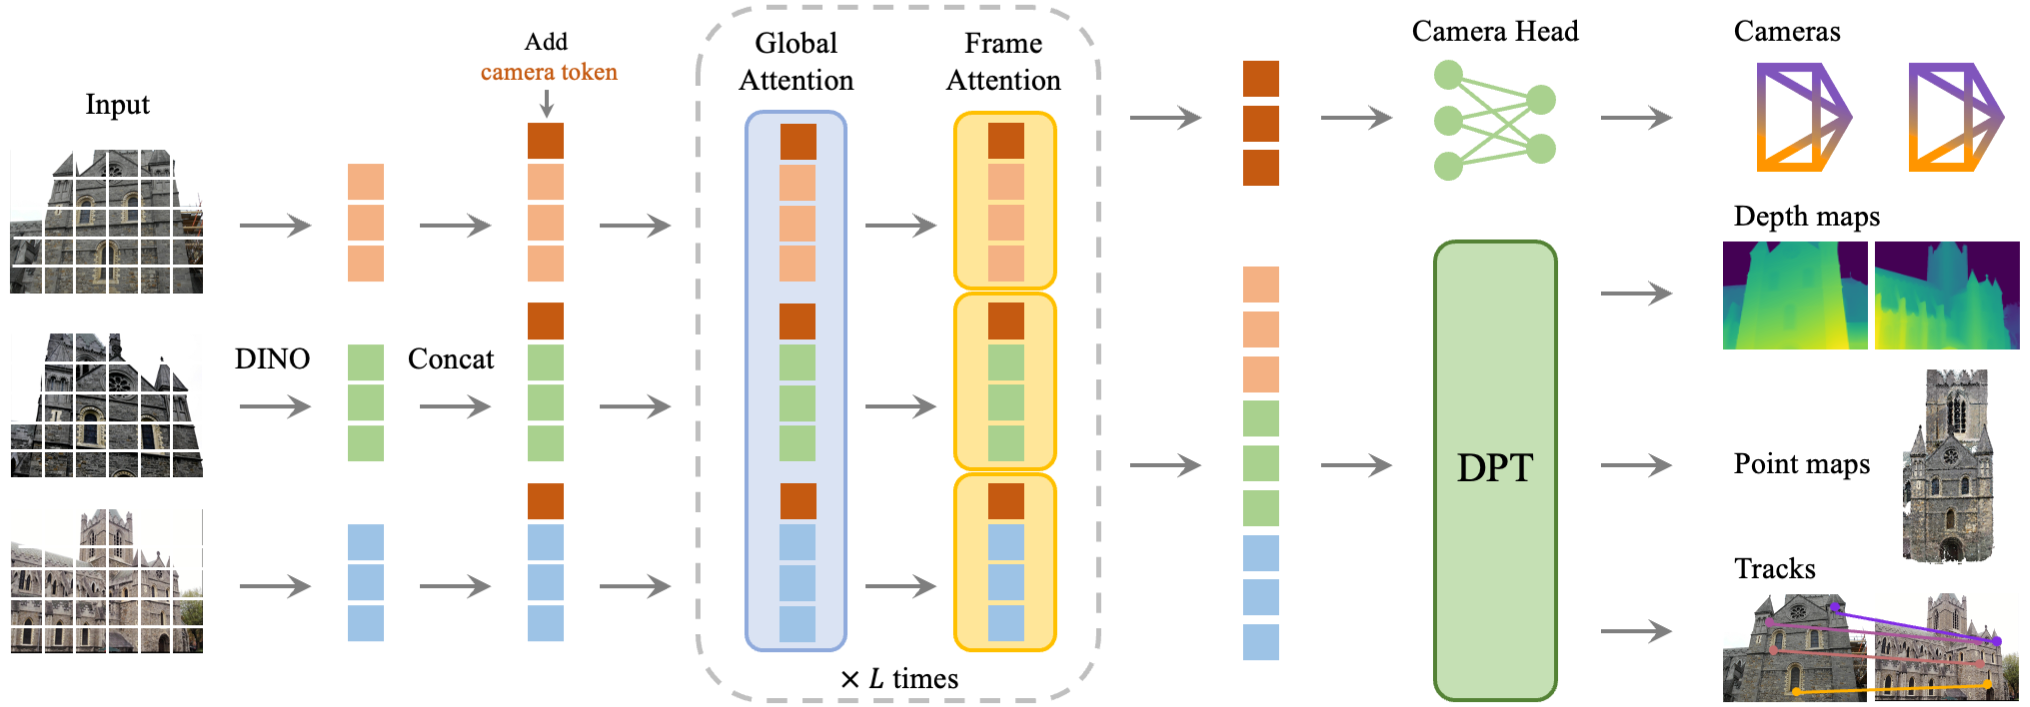
\includegraphics[width=0.65\linewidth]{vggt_architecture.png}
		\caption{Kiến trúc VGGT nhận đầu vào nhiều ảnh và dự đoán thông tin 3D.}
	\end{figure}
\end{frame}

%----------------------------------------------------------------------------------------

\section{Mục tiêu nghiên cứu}

% SLIDE 5
\begin{frame}
	\frametitle{Mục tiêu nghiên cứu}
	
	\textbf{Mục tiêu tổng quát:} Xây dựng và kiểm chứng quy trình sử dụng tín hiệu VGGT để đánh giá và hiệu chỉnh tính nhất quán hình học 3D của bản đồ độ sâu video.
	
	\vspace{0.5cm}
	\textbf{Ba mục tiêu cụ thể:}
	\begin{enumerate}
		\item \textbf{Chuẩn hóa:} Xây dựng quy trình chuẩn hóa bản đồ độ sâu, camera, điểm theo dõi từ VGGT (căn chỉnh tỉ lệ và độ lệch thống nhất, xử lý vùng động/che khuất).
		\item \textbf{Chỉ số đánh giá:} Đề xuất và kiểm chứng 3 nhóm chỉ số (độ ổn định vị trí 3D, sai số chiếu lại dài hạn, độ trôi tỉ lệ/độ lệch) đối chiếu với dữ liệu chuẩn.
		\item \textbf{Hiệu chỉnh:} Xây dựng thử nghiệm thích nghi thời điểm kiểm thử (test-time adaptation) ở đầu ra bằng biến đổi affine mà không cập nhật trọng số.
	\end{enumerate}
\end{frame}

%----------------------------------------------------------------------------------------

\section{Nội dung và phương pháp}

% SLIDE 6
\begin{frame}
	\frametitle{Phạm vi, đầu vào và đầu ra}
	
	\begin{columns}[t]
		\begin{column}{0.5\textwidth}
			\textbf{Phạm vi \& Đối tượng}
			\begin{itemize}
				\item Mô hình độ sâu: \textbf{Video Depth Anything} (chính).
				\item Tín hiệu hỗ trợ: \textbf{VGGT}.
				\item Không huấn luyện lại mô hình từ đầu.
			\end{itemize}
		\end{column}
		\begin{column}{0.5\textwidth}
			\textbf{Dữ liệu kiểm chứng}
			\begin{itemize}
				\item \textbf{TUM RGB-D}: Dữ liệu RGB-D thực tế, có quỹ đạo camera.
				\item \textbf{Sintel}: Dữ liệu tổng hợp, có ground truth đầy đủ.
			\end{itemize}
		\end{column}
	\end{columns}
	
	\vspace{0.5cm}
	\begin{block}{Đầu vào và Đầu ra}
		\begin{itemize}
			\item \textbf{Đầu vào:} Video ngắn (8-64 khung hình), độ sâu cần đánh giá, dữ liệu VGGT. (Dữ liệu chuẩn chỉ dùng để kiểm chứng).
			\item \textbf{Đầu ra:} 3 nhóm chỉ số, bảng so sánh giữa hai giao thức, đồ thị độ nhạy, và kết quả độ sâu trước/sau hiệu chỉnh.
		\end{itemize}
	\end{block}
\end{frame}

% SLIDE 7
\begin{frame}
	\frametitle{Quy trình nghiên cứu}
	
	Quy trình gồm 4 bước, so sánh song song giữa giao thức VGGT và giao thức tham chiếu (Ground Truth):
	
	\begin{figure}
		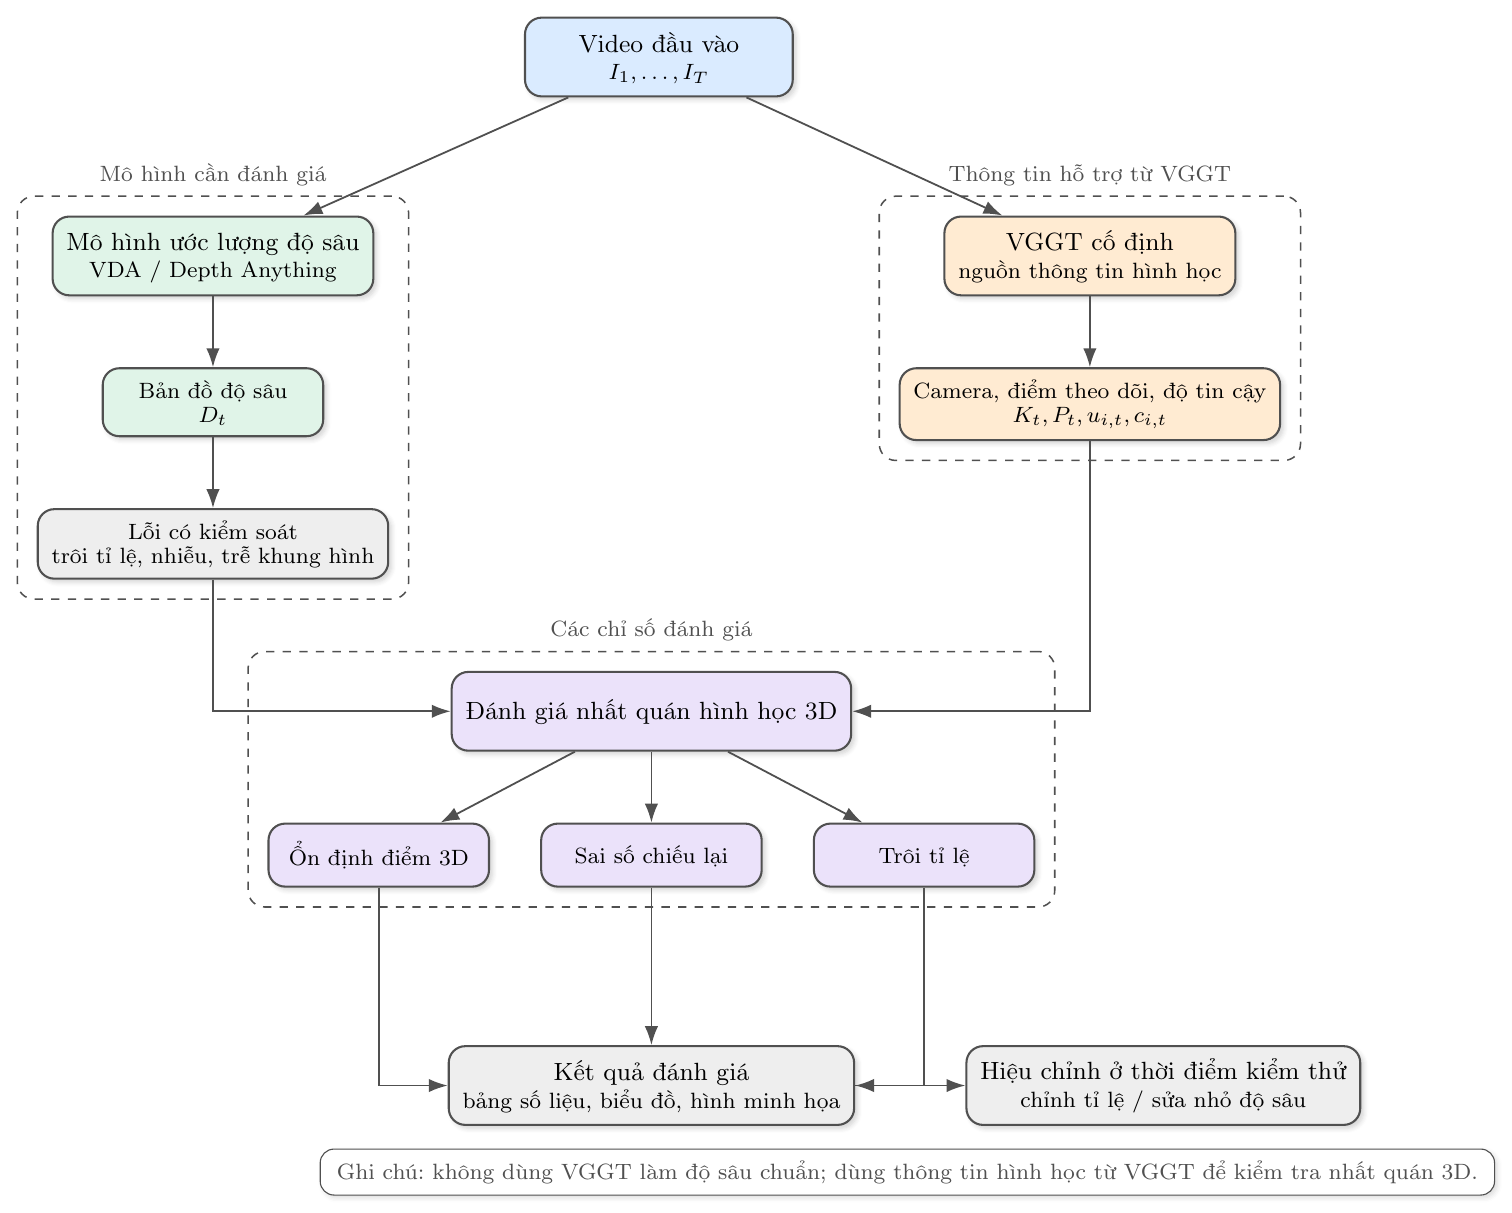
\includegraphics[width=0.85\linewidth]{proposal_pipeline_diagram.png}
		\caption{Sơ đồ tổng quát của quy trình đánh giá và hiệu chỉnh đề xuất.}
	\end{figure}
\end{frame}

% SLIDE 8
\begin{frame}
	\frametitle{Chỉ số đánh giá và kiểm chứng}
	
	\textbf{Ba nhóm chỉ số đề xuất:}
	\begin{itemize}
		\item \textbf{Độ ổn định vị trí 3D:} Đo độ phân tán vị trí 3D của các điểm thuộc quỹ đạo dài.
		\item \textbf{Sai số chiếu lại dài hạn:} Đo sai số chiếu điểm 3D qua khoảng cách thời gian xa (mở rộng so với TAE).
		\item \textbf{Độ trôi tỉ lệ và độ lệch:} Mức biến động affine theo thời gian.
	\end{itemize}
	
	\vspace{0.3cm}
	\textbf{Tiêu chí kiểm chứng (Thành công khi):}
	\begin{enumerate}
		\item Tỉ lệ xếp đúng thứ tự đạt ít nhất 80\%.
		\item Tương quan Spearman trung vị đạt $\ge 0.7$ trên 3/5 dạng sai lệch.
		\item Tương quan giữa VGGT và Ground Truth đạt $\ge 0.6$.
	\end{enumerate}
\end{frame}

%----------------------------------------------------------------------------------------

\section{Kết quả mong đợi}

% SLIDE 9
\begin{frame}
	\frametitle{Kết quả mong đợi}
	
	\begin{enumerate}
		\item \textbf{Một quy trình đánh giá có thể tái lập:} Chuẩn hóa camera, độ sâu, tính toán 3 nhóm chỉ số đánh giá 3D.
		\vspace{0.2cm}
		\item \textbf{Bộ kết quả kiểm chứng định lượng:} Bảng so sánh, biểu đồ độ nhạy, so sánh trực tiếp mức tăng lỗi với TAE, AbsRel, RMSE trên TUM RGB-D và Sintel.
		\vspace{0.2cm}
		\item \textbf{Phân tích rủi ro và giới hạn:} Điều kiện sử dụng an toàn, ảnh hưởng của vùng động và mức độ che khuất đến độ tin cậy của VGGT.
		\vspace{0.2cm}
		\item \textbf{Thử nghiệm Test-time Adaptation:} Mức giảm trung vị sai số hình học tối thiểu 5\% mà không làm AbsRel tăng quá 5\%.
	\end{enumerate}
\end{frame}

%----------------------------------------------------------------------------------------

% SLIDE 10
\begin{frame}
	\frametitle{Tài liệu tham khảo}
	
	\begin{thebibliography}{99} 
		\footnotesize 
		
		\bibitem[Wang et al., 2025]{p1}
			Jianyuan Wang, Minghao Chen, Nikita Karaev, et al. (2025)
			\newblock VGGT: Visual Geometry Grounded Transformer.
			\newblock \emph{CVPR}, 5294-5306.
			
		\bibitem[Chen et al., 2025]{p2}
			Sili Chen, Hengkai Guo, Shengnan Zhu, et al. (2025)
			\newblock Video Depth Anything: Consistent Depth Estimation for Super-Long Videos.
			\newblock \emph{CVPR}, 22831-22840.

		\bibitem[Yang et al., 2024]{p3}
			Lihe Yang, Bingyi Kang, Zilong Huang, et al. (2024)
			\newblock Depth Anything V2.
			\newblock \emph{NeurIPS}.
			
		\bibitem[Yang et al., 2025]{p4}
			Honghui Yang, Di Huang, Wei Yin, et al. (2025)
			\newblock Depth Any Video with Scalable Synthetic Data.
			\newblock \emph{ICLR}.
	\end{thebibliography}
\end{frame}

%----------------------------------------------------------------------------------------

\end{document}